
\begin{figure}
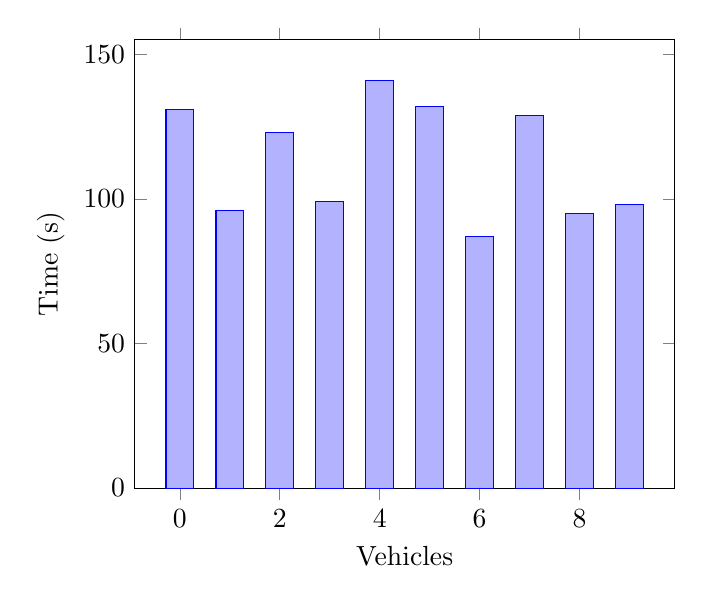
\begin{tikzpicture}
\begin{axis}[
legend style={anchor=west},
xlabel=Vehicles,
ylabel=Time (s),
ymin=0,
ybar,
]
\addplot coordinates {
(0, 131)
(1, 96)
(2, 123)
(3, 99)
(4, 141)
(5, 132)
(6, 87)
(7, 129)
(8, 95)
(9, 98)
};

\end{axis}
\end{tikzpicture}
\label{tik:100:1_S, 1_S.-60, 4_S, 5_S, 5_S.-30, 7_S, 7_S.-25, 11_S, 11_S.-50, 12_V}
\caption{100 percent diving with GSC on route $1_S, 1_S.-60, 4_S, 5_S, 5_S.-30, 7_S, 7_S.-25, 11_S, 11_S.-50, 12_V$}
\end{figure}
